\documentclass[10pt, letterpaper]{report}
% !TeX program = xelatex
%==================PREAMBOLO=======================%
\input{../../preamble/preamble.tex}
\newcommand{\titolo}{Robotics 1 }

 %TOGLI COMMENTO SE USI XELATEX
%\usepackage{fontspec}
\title{\titolo} %========TITOLO========%
\author{Marco Casu}
\date{\vspace{-5ex}}
\begin{document}

%==================COPERTINA=======================%
\begin{titlepage}
    
\begin{center}
    %TOGLI COMMENTO SE USI XELATEX
   %\setmainfont{Palace Script MT}
   \HUGE Marco Casu\acc
\end{center}
\thispagestyle{empty}
\begin{figure}[h]
    \centering{
        %l'immagine deve avere una risoluzione 2048x2048
        \includegraphics[width=1\textwidth ]{images/Copertina.png}
    }
\end{figure}
\vfill 
\centering \includegraphics[width=0.4\textwidth ]{../../preamble/Stemma_sapienza.png} \acc
\centering \Large \color{sapienza}Faculty of Information Engineering, Computer Science and Statistics\\
Department of Computer, Control and Management Engineering\\
Master's degree in Artificial Intelligence and Robotics
\end{titlepage}

%===================FINE COPERTINA======================%
\newpage
%\pagecolor{cartaRiciclata}%\setmainfont{Algerian}
\Large
This document summarizes and presents the topics for the \titolo course for the Master's degree in Artificial Intelligence and Robotics at Sapienza University of Rome. The document is free for any use. If the reader notices any typos, they are kindly requested to report them to the author.
\vfill
\begin{figure}[h!]
    \raggedright
    \includegraphics[width=0.4\textwidth,right ]{../../preamble/tomodachi.pdf} 
\end{figure}
\newpage %\setmainfont{Times New Roman}
\normalsize

\tableofcontents 
\newpage

%==================FOOTER e HEADER=======================%
\fancyhf{}
\fancyhead[L]{\nouppercase{\leftmark}}
\fancyhead[R]{Sezione \thesection}
\fancyfoot[C]{\thepage}
\fancyfoot[L]{\titolo}
\fancyfoot[R]{ Marco Casu}
%\fancyfoot[R]{\setmainfont{Palace Script MT}\huge Marco Casu \setmainfont{Times New Roman}}
%==================FOOTER e HEADER=======================%

%==================INIZIO======================%
\chapter{Introduction}
In this chapter we will see a brief introduction to the mathematical tools used in the main topics of the course. The topics presented in this section may seem somewhat unclear, as many concepts and definitions are only briefly introduced and deliberately not elaborated upon. They will be discussed in detail in their respective chapters.\bigskip
\section{About the End Effector Pose}
A robot is made up of a series of arms connected to one another by joints, these joints can be \textbf{revolut} or \textbf{prismatic} (as shown in figure \ref{img:joints}), a revolut joint rotate the link connected along 1 axis, the prismatic joint can make the link extend or contract, making them translate along 1 axis.

\begin{figure}[h!]
    \centering
    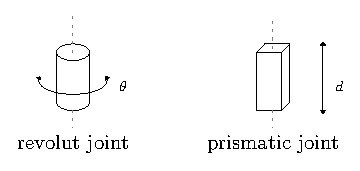
\includegraphics[width=0.6\textwidth ]{images/joints.eps} 
    \caption{two types of joints (spatial representation)}
    \label{img:joints}
\end{figure}

It is important to know that that if the angle $\theta$ increase the joint is rotating counter clock wise. In a planar drawing, the joints are denoted as shown in image \ref{img:joints_planar}.

\begin{figure}[h!]
    \centering
    \includegraphics[width=0.6\textwidth ]{images/joints_planar.eps} 
    \caption{planar representation of the joints}
    \label{img:joints_planar}
\end{figure}

In the mathematical/geometrical model of a robotic arms, it is important the \textit{kinematic skeleton}, the quantities involved are\begin{itemize}
    \item the current angle of the joints
    \item the length of the links
\end{itemize}
everything is defined respect to the base frame, usually denoted as $\Sigma_0$.

\begin{figure}[h!]
    \centering
    \includegraphics[width=0.45\textwidth ]{images/spatial_robot_new.eps} 
    \caption{spatial R4 robot}
    \label{img:spatialR4}
\end{figure}
\bigskip

The robot shown in figure \ref{img:spatialR4} is an \textit{R4 robot} (4 revolut joints) with three links. With ${}^0\mathbf p_e$ and $\Sigma_e$ we denote the position and the reference frame of the \textbf{end effector}, if there are a 0 supscript to a vector, we mean that is expressed in the base reference frame.\bigskip

With \textbf{Direct Kinematics}, we define the problem to find what are the \textbf{pose} (position and orientation) of the end effector, in function of the joint's angles. \begin{align}
    &Kin_p(\boldsymbol{\theta}):\Sigma_0\rightarrow\Sigma_e\\
    &\boldsymbol{\theta}=\begin{pmatrix}
        \theta_1&\theta_2&\theta_3&\theta_4
    \end{pmatrix}^T
\end{align}
With $\Sigma_e$ is denoted the reference frame of the end effector. How can we compute $Kin_p(\boldsymbol{\theta})$? This is given by an homogeneous $4\times 4$ matrix defined as follows:\begin{equation}
    {}^0T_e=\begin{pmatrix}
        & & & \\
        & {}^0R_e & &{}^0\mathbf p_e \\
        & & & \\
        0& 0&0 &1 
    \end{pmatrix}
\end{equation}
where\begin{itemize}
    \item ${}^0R_e\in SO(3)$ is the rotation matrix, and depends from $\boldsymbol{\theta}$
    \item ${}^0\mathbf p_e\in \R^3$ is the translation vector.
\end{itemize}

\noindent\textbf{Recall}: $SO(3)$ is the group of all the orthogonal $3\times 3$ matrices with determinant equals to 1.\bigskip

\noindent The matrix ${}^0T_e$ is obtained by multiplying $n$ matrix (where $n$ is the number of joints)\begin{align}
     &{}^0T_e= {}^0A_1(\theta_1) {}^1A_2(\theta_2)\dots {}^{n-1}A_n(\theta_n)=\\&\prod_{i=0}^{n-1}{}^iA_{i+1}(\theta_{i+1}).
\end{align}
Each \textit{homogeneous matrix} $^{i-1}A_i$ describe the pose of the $i$-th joint's frame respect to the previous joint's frame, and depends from $\theta_i$ (the $i$-th joint's angle). A more detailed description of the matrix describing the direct kinematics will be given later.\bigskip


If there are another frame $\Sigma_w$, the new matrix can be computed as follows\begin{equation}
    {}^w T_e={}^w T_0{}^0 T_e.
\end{equation}\begin{center}
    \includegraphics[width=0.8\textwidth ]{images/T_matrix_new.eps} 
\end{center}

The \textbf{Inverse Kinematics} is the opposite problem, given a position ${}^0\mathbf p_e$ for the end effector, we want to find the values of $\boldsymbol\theta$ such that\begin{equation}
    {}^0\mathbf p_e=Kin_p(\btheta)
\end{equation}
to find $\btheta$, we have to solve a non-linear system of equations, this is generally an undecidable problem, but for some specific cases, there exists a closed form, that can be found analytically, there are also numerical methods. Clearly, for the positions out of the work space, the system does not admit solutions (also this can be checked analytically).
\section{About the End Effector Velocity}
Let's now consider \textbf{Differential Kinematics}, that is the problem to find the end effector velocity in the workspace given the velocity of the joint's angles. 
Since the superposition principle is valid, the components resulting from the movement of each individual joint, which constitute the final velocity of the end effector, can be considered separately. It is important to know that the velocity component of the end effector given by a joint, is always orthogonal to the rotation axis of that joint.\bigskip

\noindent The end effector have\begin{itemize}
    \item a linear velocity, usually denoted $\mathbf v$
    \item an angular velocity, usually denoted $\bomega$.
\end{itemize}
\begin{figure}[h!]
    \centering
    \includegraphics[width=0.28\textwidth ]{images/velocity_new.eps} 
    \caption{possible trajectory by moving $\theta_1$}
    \label{img:velocity_trajectory}
\end{figure}

In the figure \ref{img:velocity_trajectory} the curve $\gamma$ represent all possible positions where the end effector could lie if the angle $\theta_1$ change, the linear velocity of the end effector is orthogonal to the $z_0$ axis. The velocity of the end effector doesn't depend only from the angular velocity, but also from the current configuration of the angles $\btheta$.\bigskip

Even if the end effector is a rigid body, is sufficient to know the linear velocity of only one point and his angular velocity to compute the velocity of all the other points, since the following relation holds:\begin{equation}
    \mathbf v_2 = \mathbf v_1+\bomega\times \mathbf r_{12}
\end{equation}
where\begin{itemize}
    \item $\mathbf v_1$ is the velocity of the first point
    \item $\mathbf v_2$ is the velocity of the second point
    \item $\bomega$ is the angular velocity of the rigid body
    \item $\mathbf r_{12}$ is the difference between the positions of the two points.
\end{itemize}
Let's analyze the velocity components of the end effector. If the $i$-th joint is changing is angle, the linear velocity of the end effector will have one component that is\begin{equation}
    \mathbf v_i=\mathbf j_i(\btheta)\dot\theta_i
\end{equation}
where $\mathbf j_i$ is a 3 components vector describing the direction of the velocity.
Since the direction depends from the configuration, the vector $\mathbf j_i$ is in function of $\btheta$.
This holds for all the angles $\theta_i$, the resultant linear velocity of the end effector will be\begin{equation}
    \mathbf v=\sum_{i=1}^n\mathbf j_i(\btheta)\dot\theta_i
\end{equation}
it can be written in matrix form\begin{equation}
    \mathbf v = J_L(\btheta)\dot\btheta=\begin{pmatrix}
        &&\\
        \mathbf j_1(\btheta)&\dots&\mathbf j_n(\btheta)\\
        &&
    \end{pmatrix}\begin{pmatrix}
        \dot\theta_1\\\dot\theta_2\\\dot\theta_3
    \end{pmatrix}
\end{equation}
where $J_L(\btheta)$ is a $3\times n$ matrix called the \textbf{Jacobian Matrix}, where $n$ is the number of joints. This description were given in terms of the linear velocity, but it holds also for the angular velocity of the end effector, indeed we have two Jacobian Matrix:\begin{itemize}
    \item we denote $J_L(\btheta)$ the Jacobian matrix for the linear velocity
    \item we denote $J_A(\btheta)$ the Jacobian matrix for the angular velocity\begin{equation}
        \bomega=J_A(\btheta)\dot\btheta
    \end{equation}
\end{itemize}
the matrix\begin{equation}
    J(\btheta)=\begin{pmatrix}
        J_L(\btheta)\\
        J_A(\btheta)
    \end{pmatrix}\in Mat(6\times n)
\end{equation}
it's called \textbf{basic Jacobian}.\bigskip

The Jacobian matrix is a mapping from the joint velocity space to the end effector velocity space. Let's ignore the angular velocity for now, suppose that we want to impose to the end effector a desired linear velocity (in a specific time instant)\begin{equation}
    \mathbf v=\mathbf v_d\in\R^3
\end{equation}
we need to find the values for the vector $\dot\btheta$ such that \begin{equation}\label{eq:diff_inv_kin}
    \mathbf v_d=J_L(\btheta)\dot\btheta
\end{equation}
if we have 3 joints, the matrix $J$ is squared and can be inverted\begin{equation}
    \dot\btheta=J_L^{-1}(\btheta) \mathbf v_d
\end{equation}
but this is not the general case, if $n>3$, the system of equations given in \eqref{eq:diff_inv_kin} could\begin{itemize}
    \item have zero solutions
    \item have infinite solutions
\end{itemize}
if the determinant of $J_L^{-1}$ is zero, the system admit infinite solutions if and only if the desired velocity vector $\mathbf v_d$ is in the range space of $J_L^{-1}$\begin{equation}
    \det J_L^{-1}=0\implies \exists \text{ inf. sol. }\iff   \mathbf v_d\in \text{Range}(J_L^{-1})
\end{equation}
we remind that the range space of a matrix, is the set of all the linear combinations of the matrix's columns. If this isn't true, the system does not admit any solution, it means that no possible combination of velocity $\dot\btheta$ could realize the desired end effector velocity. 
\subsection{Singularity}
Let's talk about \textbf{singularities} in the joint velocity space, we will give a geometric example. Let's consider a 2R planar robot, with a fixed joints configuration $\btheta$, the Jacobian is a $2\times 2$ matrix. Let $\mathbf v_d$ to be the desired velocity, the system is the following\begin{equation}
    \begin{pmatrix}
        v_d^x\\v_d^y
    \end{pmatrix}=
    \begin{pmatrix}
       \mathbf j_1^T\\\mathbf j_2^T
    \end{pmatrix}
    \begin{pmatrix}
        \dot\theta_1\\\dot\theta_2
    \end{pmatrix}
\end{equation}
the two linear equation of the system is represented on the plane as two lines. If $\det J_L\ne 0$, there are only one solution, and is the intersection between the two lines.
\begin{center}
    \includegraphics[width=0.4\textwidth ]{images/system_one_sol.eps} 
\end{center}
If $\det J_L= 0$, the two lines are parallel, so either they have no intersection, or they are the same line. If there are infinite solutions, we can choose the one with the smallest norm, since represents the ''minimum energy'' solution (the solution that requires the least joint rotation speed intensity).
\begin{center}
    \includegraphics[width=0.4\textwidth ]{images/infinite_sol.eps} 
\end{center}
We have a \textit{singularity} when the determinant approaches zero\begin{equation}
    \det J_L\rightarrow 0
\end{equation}
The closer the determinant (in absolute value) gets to zero, the more "nearly" parallel the row vectors (and thus the lines they represent) become, which means the angle of intersection approaches zero. In this case the norm of the solution could be large.
\begin{center}
    \includegraphics[width=0.4\textwidth ]{images/singularity.eps} 
\end{center}
This is true also because the following relations holds
\begin{align}
    &J_L=\begin{pmatrix}
        j_{11}&j_{12}\\
         j_{21}&j_{22}
    \end{pmatrix}\implies\\ &J_L^{-1}=\frac{1}{\det J_L}\begin{pmatrix}
        j_{22}&-j_{12}\\
         -j_{21}&j_{11}
    \end{pmatrix}\\
    &\mathbf v_d=J_L\dot\btheta\\
    &\dot\btheta=J_L^{-1}\mathbf v_d\\
      &\dot\btheta=\frac{1}{\det J_L}\begin{pmatrix}
        j_{22}&-j_{12}\\
         -j_{21}&j_{11}
    \end{pmatrix}\mathbf v_d
\end{align}
with $\det J_L\rightarrow 0$ the term $\frac{1}{\det J_L}$ (and with it, also $\dot\btheta$) became bigger and bigger. In this case, the required joint rotation velocity might not be achievable by the robotic arm's motors.\bigskip

The previous example showed how certain algebraic relationships are connected to physical problems in robot joint control. Another similar example is the following, consider the robotic arm shown in figure \ref{img:impossible_traj}.

\begin{figure}[h!]
    \centering
    \includegraphics[width=0.4\textwidth ]{images/impossible_velocity_new.eps} 
    \caption{3R spatial robot}
    \label{img:impossible_traj}
\end{figure}

Geometrically, it can be seen that by rotating only the first joint $\theta_1$, the position of the end effector will not change, this condition holds when\begin{equation}
    J_L(\btheta)\begin{pmatrix}
        \dot\theta_1\\0\\0
    \end{pmatrix}=\begin{pmatrix}
        0\\0\\0
    \end{pmatrix}
\end{equation}
this is true if the vector $\begin{pmatrix}
        \dot\theta_1&0&0
    \end{pmatrix}^T$ is in the kernel of the Jacobian matrix\begin{equation}
        \begin{pmatrix}
        \dot\theta_1\\0\\0
    \end{pmatrix}\in \ker J_L(\btheta).
    \end{equation}
\end{document}